\documentclass[dvisvgm,border=2pt]{standalone}
% Shared by every figure. Two colours only: black becomes the text colour of
% whatever theme the app is in, and `accent` becomes the brand — see
% scripts/build-figures.mjs. Everything else is done with opacity.
\usepackage{amsmath}
\usepackage{amssymb}
\usepackage{tikz}
\usepackage{pgfplots}
\pgfplotsset{compat=1.18}
\usetikzlibrary{arrows.meta,positioning,calc,backgrounds,fit,patterns.meta}
\definecolor{accent}{RGB}{255,0,255}
\pgfplotsset{
  every axis/.append style={
    axis lines=left,
    axis line style={draw opacity=0.35},
    tick style={draw opacity=0.35},
    tick label style={font=\scriptsize,opacity=0.7},
    label style={font=\scriptsize,opacity=0.7},
    legend style={draw=none,fill=none,font=\scriptsize},
    every axis plot/.append style={line width=0.7pt},
  },
}
\tikzset{
  every picture/.style={font=\scriptsize},
  faint/.style={opacity=0.3},
  quiet/.style={opacity=0.55},
  box/.style={draw,opacity=0.35,rounded corners=2pt,inner sep=4pt},
  hot/.style={accent},
}

\begin{document}
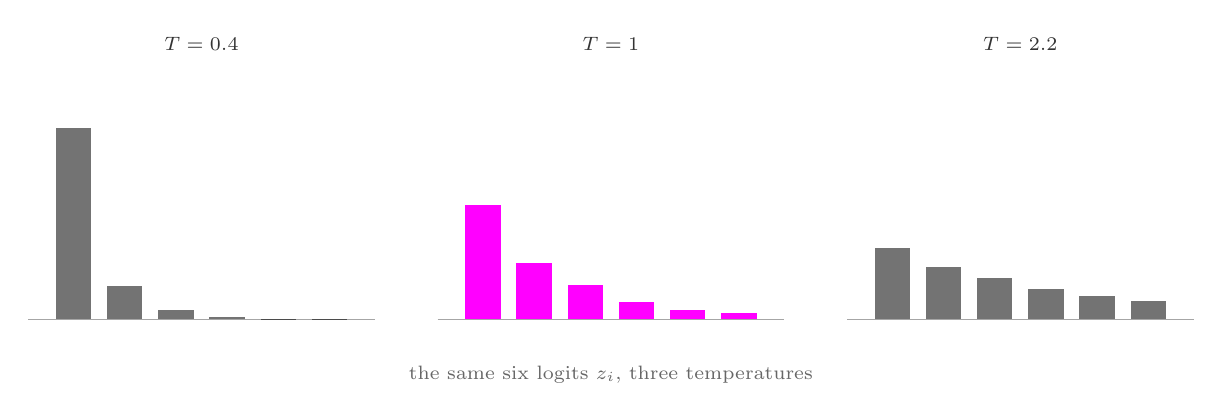
\begin{tikzpicture}
  \foreach \T/\dx/\lab/\sty in {0.4/0/{$T=0.4$}/quiet,
                                1.0/5.2/{$T=1$}/hot,
                                2.2/10.4/{$T=2.2$}/quiet}{
    \begin{scope}[xshift=\dx cm]
      \draw[opacity=0.35] (0,0) -- (4.4,0);
      \node[opacity=0.8] at (2.2,3.5) {\lab};
      \foreach \z [count=\i from 0] in {3.1,2.4,1.9,1.2,0.6,0.1}{
        \pgfmathsetmacro{\num}{exp(\z/\T)}
        \pgfmathsetmacro{\den}{exp(3.1/\T)+exp(2.4/\T)+exp(1.9/\T)+exp(1.2/\T)+exp(0.6/\T)+exp(0.1/\T)}
        \pgfmathsetmacro{\p}{\num/\den}
        \fill[\sty] (0.35+\i*0.65,0) rectangle ++(0.45,3.0*\p);
      }
    \end{scope}
  }
  \node[opacity=0.6] at (7.4,-0.7) {the same six logits $z_i$, three temperatures};
\end{tikzpicture}
\end{document}
